\label{sec:l2}
Die paarweise Kollisionserkennung bezieht sich auf die Kollision von genau zwei 3D-Modellen in ihrer exaktesten Darstellung. Die Genauigkeit der Kollisionserkennung bei steigender Modellkomplexität ist hier im Fokus.

\subsection{Input}
Aus den in Abschnitt \ref{sec:l1} beschriebenen Verfahren wird eine Menge von Objektpaaren erhalten, für die eine Kollisionsvermutung während eines Ticks gilt $C_{guess}\subseteq OBJ^2$. Es ist gefordert, dass die Menge der tatsächlichen Kollisionen in der Menge der vermuteten, vorgefilterten Kollisionspaare vollständig enthalten ist $C_{definitive}\subseteq C_{guess}$.\\
Beim Simulationsprozess eines Objektes wird der Status des Objektes auf einen neuen, späteren, gewünschten Zeitpunkt gehoben.\\
Zum Objekt angegeben ist sein Zustand zum Simulationszeitpunkt des letzten an ihm durchgeführten Simulationsschritts. Zur Zustandsinformation gehören:
\begin{itemize}
\item der Simulationszeitpunkt dieser letzten Aktualisierung
\item das Modell\\
Modelle von Objekten werden als Polygon-Mesh \cites{fourcrossfour}{ogl} angegeben, welche einen Polyeder beschreiben. Es ist von Algorithmen gefordert eine theoretische kompakte Punktemenge von Objekten semantisch zu berücksichtigen (siehe Anhang \ref{sec:object_form}).
\item Platzierung (siehe Anhang \ref{sec:objects_sim})
\begin{itemize}
\item Position
\item Rotation
\end{itemize}
\item Bewegung\\
Diese ist konstant während eines Ticks und wird zu Ende eines solchen, oder bevorzugt von Interaktionsroutinen, wie der Kollisionsroutine, aktualisiert.
\begin{itemize}
\item Geschwindigkeit $v$
\item Winkelgeschwindigkeit $\omega$
\end{itemize}
\end{itemize}

Die Objektstatus der Objekte werden zu einem der Objekte im eingegeben Paar relativiert.  Die Positionen, welche das Objekt zu anderen Zeiten $t$ des Simulationsschrittes einnimmt, werden durch Transformationen der Objektform ermittelt. Für weiter Details können die Anhänge \ref{sec:space} und \ref{sec:object_sim} herangezogen werden.\\

\subsection{Output}
Es ist eine Aufgabe des modellgenauen Kollisionsschritt, sämtliche restlichen False-Positives aus dem Schritt der Kollisionspaarvorfilterung zu eliminieren.
Eine zweite Aufgabe ist die Ermittlung von Informationen über den Hergang von Kollisionen.
Im Abschnitt~\ref{sec:usages} werden einige für dieses Projekt interessante Verwendungszwecke der Kollisionsermittlung aufgelistet, welche unterschiedliche Anforderungen hinsichtlich benötigter Information über den Kollisionsvorgang haben, um realisiert werden zu können:
\begin{enumerate}
	\item Schnitt\\
		Die Frage ob Objekte sich an einem konkreten Zeitpunkt während eines Ticks schneiden/gegenseitig enthalten.
	\item Intrusion\\
		Die Frage nach den Eigenschaften
		\begin{enumerate}
		\item ob
		\item zu welchem Simulationszeitpunkt
		\item an welcher Raumposition
		\item mit welchen Teilen des Objektes/ an welcher Position am Objekt
		\end{enumerate}
		ein Eindringen eines Objektes in ein anderes stattfindet, d.h. ein Zustandsübergang von Nicht-Schnitt zu Schnitt stattfindet.
\end{enumerate}
Für physikalische Verwendungszwecke, insbesondere bei der rigiden Objektkollision, erscheint Intrusion besonders interessant. Der aktive Zustand des Schnitts zweier kollisionsfähiger Entitäten/Objekte soll prinzipiell nicht erlaubt sein und muss daher aktiv durch eine Kollisionsreaktion zum Zeitpunkt der Erstkollision verhindert werden.\\
Die derzeitig geforderte Reaktion von Objekten auf Kollision ist der Stillstand ($v = \omega = 0$) zum kollidierenden Zeitpunkt. Die Umsetzung der Auflösung von Kollisionen und Mehrfachkollisionen ist explizit aus diesem Projekt ausgeschlossen. Selbst jedoch bei der rudimentären theoretischen Betrachtung von Mehrfachkollisionen während eines Ticks und Optionen zu deren Auflösung, bzw.~physikalischer Reaktion von Objekten, scheinen vorwiegend Erstkollisionen interessant zu sein.\\
Aus Algorithmen für Erstkollisionen kann adaptiv zu einem späteren Zeitpunkt eine Mehrfachkollisionsroutine durch sukzessive Aufrufe realisiert werden. Ob dieses Vorgehen von Vorteil ist soll an dieser Stelle nicht entschieden werden.

\subsection{Intrusionsermittlung mithilfe geometrischer Berechnungen am durchlaufenen Volumen bei linearer Bewegung}
\label{sec:linear_int}
Bei diesem Verfahren soll das durchlaufenen Volumen von Objekten abgeprüft werden, während diese eine lineare Bewegung ausführen. Die Punkte der Kollision zweier durchlaufener Volumen sollen zur Ermittlung weiterer Informationen zum Ablauf der Kollision verwendet werden. Wir sehen ähnliche Ansatze zur Kollisionsermittlung bei linearen Bewegungen idealisiert in Quelle \cite[ch.12, p.361]{fourcrossfour} und schätzen den Ansatz daher als vernünftigen, relativ simplen, ersten Versuch ein, Kollisionserkennung in einem beschränkten Rahmen umzusetzen.
\subsubsection{Verwendungszweck und Limitation}
Der hier vorgestellte Algorithmus behandelt Objekte so als würden sie während eines Ticks keine zeitliche Änderung der Rotation erfahren.\\
Dies hat mehrere Gründe:
\begin{enumerate}
\item Objekte (bzw. Entitäten) hielten zum Start des Projekts noch keine Repräsentation für Rotation.
\item Rotation in einer Kollisionsroutine mit einzubeziehen wird schon früh im Projekt als schwierig eingeschätzt. Dieser Verhalt sollte sich später bestätigen.
\item Es gibt ausreichend Kollisionsszenarien/Verwendungszwecke bei denen Rotation keine Rolle spielen muss (Logische Kollision, punktförmige Objekte, unbewegliche Objekte wie z.B. oft Terrain, Verwendungszwecke mit hoher Fehlertoleranz). Ein solcher Algorithmus ist also von Wert.
\item Durch die Vernachlässigung von $\omega$ werden die Bewegungen von Objekten linear. Das den weiteren entscheidenden Vorteil, dass bei einer Relativierung der Objekte wechselseitig zueinander, eine Operation der einer Transformation in Form einer Translation gleichkommt, die Linearität weiterhin gewahrt bleibt. Zum Vergleich: Mit aktiver Rotation beschreiben Objekte relativ zueinander Kurvenflugbahnen, welche sehr viel schwerer zu berechnen und damit zu interpolieren sind.\\
\end{enumerate}

\subsubsection{Umsetzung}
Alle im Objekt $o$ enthaltenen Punkte $p \in K_o$ beschreiben lineare, zueinander parallele Flugbahnen während der Simulationszeitsequenz eines Ticks $\Upsilon_{\delta_i}$:
$$l_p = \{ p + (t - t_0) \cdot v(o, t_0) | t \in \Upsilon_{\delta_i} \}$$
In ihrer Gesamtheit beschreiben diese das durchlaufene Volumen des Objekts:
$$\{l_p|p\in K_o\} = \{K_{o, t}| t \in \Upsilon_{\delta_i}\}$$

Durch die Relativierung der Objektzustände beider Objekte zu einem Zustand eines der eingegebenen Objekte muss nur für jeweils das andere Objekt diese lineare Erweiterung für einen konkreten Kollisionstest berechnet werden. Das gilt auch für alle Poleder-Merkmale der Objekte.\\
Die Merkmale des Polyhydra des Objekts $o$ sind:
\begin{itemize}
\item Ecken $V_o$
\item Kanten $E_o$
\item Flächen $A_o$
\end{itemize}
Modelle sind als Polyeder angegeben, welche mindestens die Objekthülle zur kompakten Modellrepräsentation angibt. Bei zwei Objekten $o_0, o_1$, zeitlich bevor ein innerer Punkt $K_{o_1} \setminus (V_{o_1} \cup E_{o_1} \cup A_{o_1})$ sich mit dem anderen Objekt $K_{o_0}$ schneiden kann, müssen die Objekthüllen bereits kollidiert sein. Die semantische Äquivalenz der kompakten Modellrepräsentation und der Polyeder-Repräsentation sei damit im Kontext dieses Algorithmus hergestellt.\\

Wenn eine Dreiecksfläche linear durch die Zeit erweitert werden würde, entstünde daraus ein schiefes Prisma, was eine vergleichsweise zu den anderen Merkmalskandidaten eine  komplexe geometrische Form ist. Weiter müssen nicht alle Merkmale miteinander kollidiert werden. Durch Elimination werden die essentiell zu kollidierende Merkmalspaare aus $\{Area, Edge, Vertex\}^2$ ermittelt:
 werden  sind:
		\begin{itemize}
			\item $\{Vertex, Area\}$ Eine Ecke durchschlägt eine Fläche.\\
				$\Rightarrow$ Zu überprüfende Paare: $(V_{o_0}\times A_{o_1})\cup (V_{o_1}\times A_{o_0})$
			\item $\{Edge, Edge\}$ Kanten durchschneiden sich gegenseitig.
				$\Rightarrow$ Zu überprüfende Paare: $(E_{o_0}\times E_{o_1})\cup (E_{o_1}\times E_{o_0}) = (E_{o_0}\times E_{o_1})$
		\end{itemize}
		Alle anderen Kombinationen sind entweder in diesen beiden enthalten (z.B. $\{Vertex, Edge\}$ in 1.) oder ein Ereignis dieser beiden Szenarien muss logisch vorher passieren (z.B. 1. oder 2. muss vor $\{Edge, Area\}$ bereits passiert sein).
\ \\
		Aufgrund der Relativierung muss nur eines der Merkmale eine zeitliche Bewegung durchführen:
		\begin{itemize}
			\item $\{Vertex, Area\}$ 2 Möglichkeiten:
				\begin{itemize}
					\item Eckpunkt $v \Rightarrow$ Linie $l_v$
					\item Dreiecksfläche $a \Rightarrow$ Schiefes Prisma $ \{l_p | p \in a\}$
				\end{itemize}
				Gewählt wird der Eckpunkt, da eine simplere Berechnung folgt.
			\item $\{Edge, Edge\}$ Kante $e \Rightarrow$ Parallelogramm $\{l_p | p \in e\}$
		\end{itemize}
\ \\
		Die Kollisionsüberprüfungen der Merkmale als Parallelogramm, Dreieck und Linie können über Gleichungssysteme errechnet werden. Dabei werden Koeffizienten bekannt, durch die Kollisionszeit und Ort exakt ermittelt werden können. Wir ermitteln die Merkmalskollision mit minimalem Kollisionszeitpunkt und erhalten so die Erstkollision der Gesamtobjekte.\\
		Komplexität: $\mathcal{O}(|V_{o0}|\cdot  |A_{o1}| + |V_{o1}|\cdot |A_{o0}|$ + $|E_{o0}| \cdot  |E_{o1}|)$

Wie beschrieben kann dieses Verfahren bereits in einigen Szenarien, bei denen Rotation keine Rolle spielt, als vollständige Lösung zum Einsatz gebracht werden.\\

\subsubsection{Defizite durch die Limitation}
Durch einen Extremfall der Vernachlässigung der Rotation fällt ein weiteres Defizit des Algorithmus auf. Ist die relative Geschwindigkeit zweier Objekte gleich Null, wird aus Sicht des Algorithmus kein Volumen durchstreift. Es werden zwischen diesen Objekten dann gar keine Kollisionen erkannt, welche durch Rotation entstehen.
Man könnte versuchen dieses Problem durch statische Kollisionstests am Tickende zu lösen. Dabei wird die akkumulierte Rotationsbewegung/Rotationstransformation auf einmal ausgeführt. Vor und nach der Bewegung wird statisch eine Kollisionsabfrage berechnet.\\
Diese Anpassung brächte eigene Probleme mit sich:
\begin{enumerate}
\item Durch die akkumulierte Drehung kann eine Kollision bei schnellen Drehgeschwindigkeiten durch nur die Tests am Anfang und am Ende des Ticks komplett übersehen werden.
\item Nach der Rotationstransformation können Objekte sich im verbotenen Schnittzustand befinden.\\
Eine Idee zu Auflösung ist die Suche nach einem Zeitpunkt vor der Überschneidung, durch binäre Suche \cite[ch.6.1, p.131]{fourcrossfour} des Drehungsausschlags. Prinzipiell ist dieser Algorithmus allerdings von Anfang an für Rotation konzipiert.
\end{enumerate}

Es wird also weiter nach etablierten Lösungen gesucht, die sich dem Rotationsproblem annehmen können.

\subsection{Gilbert-Johnson-Keerthi-Distanzalgorithmus (GJK)}
\label{sec:gjk}

\begin{figure}
\centering
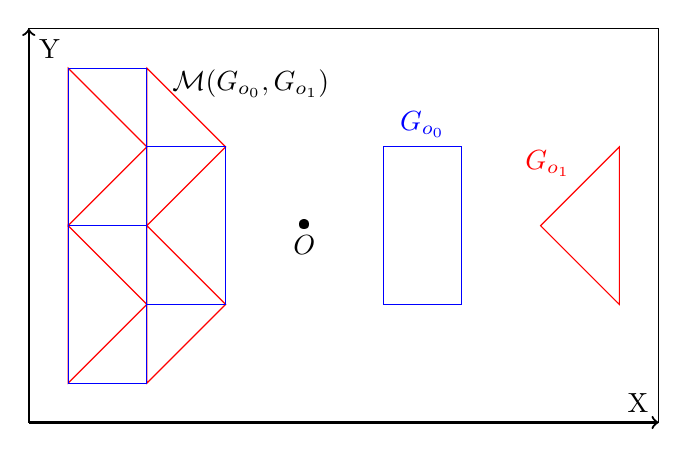
\begin{tikzpicture}

\draw (-3.5,-2.5) rectangle (4.5,2.5);
\draw[thick,->] (-3.5,-2.5) -- (4.5,-2.5) node[anchor=south east] {X};
\draw[thick,->] (-3.5,-2.5) -- (-3.5,2.5) node[anchor=north west] {Y};


\coordinate (O) at (0,0) ;
\draw [below](O) node[black]{$O$};
\draw (O) node[black]{\textbullet};

\coordinate (Ta) at (3, 0);
\coordinate (Tb) at (4, 1);
\coordinate (Tc) at (4, -1);

\draw[red] (Ta) -- node[above left]{$G_{o_1}$} (Tb) -- (Tc) -- cycle; 

\coordinate (Qa) at (1, -1);
\coordinate (Qb) at (1, 1);
\coordinate (Qc) at (2, 1);
\coordinate (Qd) at (2, -1);

\draw[blue] (Qa) -- (Qb) -- node[above]{$G_{o_0}$} (Qc) -- (Qd) -- cycle; 

\coordinate (QaTa) at (-2, -1);
\coordinate (QbTa) at (-2, 1);
\coordinate (QcTa) at (-1, 1);
\coordinate (QdTa) at (-1, -1);
\coordinate (QaTb) at (-3, -2);
\coordinate (QbTb) at (-3, 0);
\coordinate (QcTb) at (-2, 0);
\coordinate (QdTb) at (-2, -2);
\coordinate (QaTc) at (-3, 0);
\coordinate (QbTc) at (-3, 2);
\coordinate (QcTc) at (-2, 2);
\coordinate (QdTc) at (-2, -0);

\draw[red] (QaTa) -- (QaTb) -- (QaTc) -- cycle; 
\draw[red] (QbTa) -- (QbTb) -- (QbTc) --  cycle; 
\draw[red] (QcTa) -- (QcTb) -- (QcTc) -- cycle;
\draw[red] (QdTa) -- (QdTb) -- (QdTc) -- cycle;

\draw[blue] (QaTa) -- (QbTa) -- (QcTa) -- (QdTa) -- cycle; 
\draw[blue] (QaTb) -- (QbTb) -- (QcTb) -- (QdTb) -- cycle; 
\draw[blue] (QaTc) -- (QbTc) -- (QcTc) -- (QdTc) -- cycle; 

\node at (-1.8, 1.5)[above right]{$\mathcal{M}(G_{o_0}, G_{o_1})$};

\end{tikzpicture}
\caption{2D-Beispiel für eine Minkowski-Differenz $\mathcal{M}(G_{o_0}, G_{o_1})$ mit Ursprung $O$ und den als Mesh angegebenen Objekten $G_{o_0}$ und $G_{o_1}$. Gezeigte Linien dienen als Hilfestellung zur Erkennung von Einflüssen der Ursprungsobjekte auf die Differenz.}
\label{fig:gjk}
\end{figure}

GJK ist ein Algorithmus, der zwischen kompakten, konvexen Mengen $K_0, K_1 \subseteq \mathbb{R}^3$ die minimale euklidische Distanz $distance(K_0, K_1) = min\{|k_0 - k_1|~| k_0\in K_0 ; k_1 \in K_1\}$ errechnet. Er wurde 1988 publiziert \cite{gjk} und scheint heute gerne in Videospielen verwendet zu werden. Beispiele sind dabei Blizzard Entertainments Diabolo 3 \cite{gdc-physics} und Valves Half-Life 2\cite{gjk-casey}.\\

Die Urquelle \cite{gjk} beschreibt den Algorithmus umfassend mathematisch und detailliert. Es wird weiter Quellmaterial \cite{gjk-casey} mit praktischem Fokus zu Rate gezogen, um eine Implementierung umzusetzen und den Einstieg zu erleichtern.\\
Im GJK-Algorithmus sollen Eigenschaften der sogenannten Minkowski-Differenz $\mathcal{M}:\mathcal{P}(\mathbb{R}^3)^2\mapsto \mathcal{P}(\mathbb{R}^3); \mathcal{M}(K_0, K_1) = \{a - b| a\in K_0 ; b\in K_1\}$ \cite[p.195]{gjk} ausgenutzt werden.
Ein Beispiel für die Minkowski-Differenz ist in Abbildung \ref{fig:gjk} zu sehen. Die hier relevanten Eigenschaften der Minkowski-Differenz lauten wie folgt:\\
	\begin{enumerate}
		\item Die Minkowski-Differenz zweier konvexer Körper ist ebenfalls konvex.
		%\item $K_0 \cap K_1 \neq \emptyset \Rightarrow \exists a_o, b_o \in K_0 \cap K_1, a_0 \in K_0, b_0 \in K_1 : a_o = b_o \Rightarrow a_o - b_o = O \Rightarrow O \in \mathcal{M}(K_0, K_1)$
		%\item $K_0 \cap K_1 = \emptyset \Rightarrow \forall a_o\in K_0, \forall b_o\in K_1 : a_o \neq b_o \Rightarrow a_o - b_o \neq O \Rightarrow O \notin \mathcal{M}(K_0, K_1)$.
		\item Bei einem Schnitt der Eingabeobjekte ist der Ursprung in deren Minkowski-Differenz enthalten. Die Distanz bei einem Schnitt ist $0$.
		$$ K_0 \cap K_1 \neq \emptyset \Leftrightarrow O \in \mathcal{M}(K_0, K_1)	\Leftrightarrow distance(K_0, K_1) = 0 $$
		\item Die euklidische Distanz zwischen den Eingabeobjekten entspricht der Distanz ihrer Minkowski-Differenz und dem Ursprung. $$distance(O, \mathcal{M}(K_0, K_1)) = distance(K_0, K_1)$$
		\item Es werden nur positive Distanzwerte ermittelt. $$distance: \mathcal{P}(\mathbb{R}^3)^2 \mapsto \mathbb{R}^+_0$$
	\end{enumerate}
GJK selbst behandelt das Schnittproblem $ K_0 \cap K_1$, nicht das Intrusionsproblem.
Durch die Fähigkeit des Algorithmus, die Distanz zwischen zwei Objekten zu ermitteln, ist dieser jedoch ein praktisches Werkzeug, um das Intrusionsproblem ebenfalls zu lösen.
Zum Beispiel ist ein Ansatz, durch Abstraktion über einer Nullstellensuche der Distanz zwischen zwei Objekten das Intrusionsproblem abzubilden (vgl. \cite{gdc-physics}).\\
GJK eignet sich also für dieses Projekt und soll implementiert werden.\\

\subsubsection{Eingabe des Algorithmus und dessen semantische Äquivalenz zur kompakten Punktemenge}
\label{sec:gjk_equiv}
Als Eingabedaten vorliegend sind Polygon-Meshes für die Form der Objekte.
Für den Algorithmus sind Konvexität und semantische Äquivalenz zu kompakten Punktemenge gefordert.

Im generellen sind für die Eingabe-Polygon-Meshes keine Konvexität gefordert und eine entsprechende kompakte Repräsentation nicht gegeben.\\
Nicht-konvexe Objekte können in konvexe Partitionen aufgeteilt werden. Jede Partition zählt dann als eigenes Objekt gegenüber dem Algorithmus. Das erhöht die erwartete Komplexität der gesamten Kollisionsroutine mit GJK um den Grad der Partitionierung ($\mathcal{O}(|P_{o_0}|\cdot |P_{o_1}|)$).\\
Zu der Abschwächung der Komplexitätssteigerung scheint insbesondere eine minimale Partitionierung von Interesse.\\
Zusätzlich zu eigenen Überlegungen bestätigen die Quellen \cite{ARTIGAS20111968} und \cite{grelier2019minimum} die NP-Vollständigkeit, bzw. NP-Härte zusammengehöriger Probleme der minimalen konvexen Partitionierung.\\
Eine nicht minimale Partitionierung wäre zunächst auch ausreichend und auch lange Berechnungszeiten zur Partitionierung würden für rigide Objekte nur einmaligen Aufwand zum Programmstart bedeuten und wären daher nicht kritisch.\\
Bei Versuchen, Algorithmen für dieses Problem zu erstellen, wird jedoch eine weiter klare Hürde erkenntlich: Allein durch die Polygon-Mesh, sind Innen und Außenseite des Objektes prinzipiell nicht definiert.\\
Für grafische Zwecke kann dieser Bezug oft durch das sog. \textit{Winding} \cite[ch.5.6, p.121, ch.7.3]{fourcrossfour}\cite{gjk-casey} eines Dreiecks angegeben werden. Dabei wird die Reihenfolge der Angabe der Ecken eines Dreiecks konventionell festgelegt, wodurch die Richtung der Flächennormale eines Dreiecks kontrolliert werden kann, die dann Außen oder Innenseite spezifiziert.\\
Für die in dieser Projektarbeit verwendeten Testzwecke erscheint der Aufwand der Automatisierung der konvexen Partitionierung für dieses Projekt letztendlich doch zu hoch und thematisch zu fremd. Eine Konvention für ein \textit{Winding} wurde allerdings im Projekt eingeführt, nicht zuletzt, da diese die Implementierung des GJK vereinfacht.
\ \\
Die konvexe Partitionierung des Objektes wird letztendlich manuell und explizit bei Modellen durch Mengen beteiligter Eckpunkte einer Partition angegeben.\\
Ein Körper $K$ ist konvex, wenn gilt $\forall p_0, p_1 \in K, \forall x \in [0,1] : p0 + x \cdot  (p_1 - p0) \in K_o $ \cite[p.121]{morris2015finite}. Bei Entfaltung der Mesh-Repräsentation $M_o$ sind nicht alle diese Punkte enthalten. Da eine Polygon-Mesh jedoch die Eckpunkte angibt, können sämtliche Punkte zwischen Eckpunkten und sukzessive Kanten, Flächen und das restliche Volumen durch die Konvexitätseigenschaft impliziert werden. Die zusätzlich mit der Objektrepräsentation mitgelieferte konvexe Partitionierung erweitert also die verfügbare Information und schafft in dieser Hinsicht Äquivalenz zwischen Polygon-Meshes und kompakten Mengen und die Unterscheidung von Innen und Außen am Modell. Der Algorithmus kann demnach außschließlich unter Einbeziehung von Eckpunkten $V_o$ und der Partitionierung verfahren.

\subsubsection{Diskrete Minkowski-Differenz}
Eine Diskretisierung/Beschränkung auf die Information der Eckpunkte der Polygon-Mesh $V_o$ ist nach Abschnitt \ref{sec:gjk_equiv} möglich, was vorteilhafte Iterationslängen durch die Eingabe zur Folge hat ($|V_o| \ll |G_o| \ll |K_o|$).\\
In der Ausnutzung der Eigenschaften der Minkowski-Differenz muss nun allerdings der Umstand der Diskretion respektiert werden.

\begin{enumerate}
		\item Die Information einer diskreten Minkowski-Differenz verletzt die Zugrunde liegende Konvexität der Ursprungskörper nicht. Nach wie vor gilt : Die Minkowski-Differenz zweier konvexer Körper ist ebenfalls konvex.
		\item Wir beschreiben ein Simplex als durch eine Menge von Eckpunkten $s\in\mathcal{M}(V_{o_0}, V_{o_1})^n$ aufgespannte $n$-dimensionale geometrische, inhärent konvexe Form (hier: Punkt für $n=1$, Gerade $n=2$, Dreieck $n=3$, Tetraeder $n=4$). Durch die Konvexität ist die entsprechende kompakte Menge $K_s$ impliziert.
		\item Ein nächstes, in der Minkowski-Differenz enthaltene Simplex zum Ursprung hat die selbe euklidische Distanz (nach Definition) zum Ursprung wie die Minkowski-Differenz selbst.
\begin{align*}		
		s_{nearest} \subseteq \mathcal{M}(V_{o_0}, V_{o_1}) \\
		distance(O, K_{s_{nearest}}) = distance(K_{o_0}, K_{o_1})
		\end{align*}	 \cite[p. 195]{gjk}	
		\item Für den Fall des Enthaltens des Ursprungs einer Minkowski-Differenz im Kompakten, mag der Ursprung nicht direkt einer der in der diskreten Minkowski-Differenz enthaltenen Punkte sein.
		$$O \in \mathcal{M}(K_{o_0}, K_{o_1}) \nRightarrow O \in \mathcal{M}(V_{o_0}, V_{o_1})$$
		 Jedoch kann eine äquivalente Beziehung gefunden werden, indem ein Simplex aus den Punkten der diskreten Minkowski-Differenz gesucht wird, dass den Ursprung enthält/umschließt: 
		 $$O \in \mathcal{M}(K_{o_0}, K_{o_1}) \equiv \exists Simplex~s \subseteq \mathcal{M}(V_{o_0}, V_{o_1}) : O \in K_s$$

\end{enumerate}
Die diskrete Minkowski-Differenz wird trivial über zwei Schleifen errechnet($\mathcal{O}(|V_0| \cdot |V_1|)$).

\subsubsection{Struktur des Algorithmus}
Die Implementierung des GJK bezieht sich auf die Suche nach dem nächsten, bzw. umschließenden Simplex zum Ursprung und der Ermittlung seiner Distanz zum Ursprung.\\
Die Quellen \cites{gjk}{gjk-casey} beschreiben den Algorithmus für unsere Zwecke nicht Zusammenhängend genug. Die Quellen geben auch wechselseitig Einflüsse zueinander auf die Implementierung. Es lohnt sich daher, v.a.~ zu Referenzzwecken, die letztendliche Struktur des Algorithmus im Folgenden darzulegen:
\begin{enumerate}
	\item Initialisiere mit
	\begin{enumerate}
		\item der Fähigkeit, Abstände zwischen einem Simplex und dem Ursprung zu errechnen.  $distance: Simplex \times \mathcal{F}^3 \mapsto \mathcal{F}$
		\item Der diskreten Minkowski-Differenz zweier konvexer (Teil-)Objekte $o_0, o_1$ zu einem Zeitpunkt $t$: $\mathcal{M} = \mathcal{M}(V_{o_0, t}, V_{o_1, t})$
		\item beliebigem Startpunkt $s_0 \in \mathcal{M}$
		\item der Menge von maximal 4 indizierten Simplexeckpunkten, welche das derzeit bekannte Simplex angeben. Der Startpunkt ist dabei bereits das erste Simplex $s = \{s_0\}$
		\item der Suchrichtung in Richtung Ursprung $\vec{D} = -s_0$
		\item der minimalen gefundenen Distanz $d_{min} = distance(\{s_0\})$
		
	\end{enumerate}	
	\item \label{gjkstep2} \label{gjkbody} Erweitere das Simplex $s$ durch den neuen Punkt $s_{|s|}$, zur $(|s|+1)$-dimensionalen Erweiterung des Simplex durch den maximalen Punkt $v \in \mathcal{M}$ in der Suchrichtung $\vec{D}$.\\
	Das wird über das Skalarprodukt erreicht. 
	$$s_{|s|} = v \in \mathcal{M} : \vec{v} \circ \vec{D} = max\{\vec{D} \circ \vec{v_i}| v_i \in  \mathcal{M}\}$$

	\item \label{gjkstep3} Durch das Hinzunehmen des neuen Punktes $s \cup \{s_{|s|}\}$ kann eine Menge von neuen Simplices $s_{\alpha}=\mathcal{P}(s \cup \{s_{|s|}\})$ beschrieben werden. Es soll das zum Ursprung nächste Simplex mit niedrigster Dimensionalität ausgewählt werden.
	\begin{align*}
	s_{\beta} = \{\dot{s}\in s_{\alpha} | \forall \ddot{s} \in s_{\alpha}; distance(\dot{s}) \leq distance(\ddot{s})\} \\
	Simplex~s_{\gamma} \in \{\dot{s}\in s_{\beta} | \forall \ddot{s} \in s_{\beta}; |\dot{s}| \leq |\ddot{s}|\} \\
	\end{align*}
	
	\item Falls dieses nächste Simplex zum Ursprung $s_{\gamma}$ keine Distanzverbesserung erzielt ist das generell nächste Simplex zum Ursprung bereits durch $s$ erreicht.
	$$d_{min} \leq distance(s_{\gamma}, O) \Rightarrow distance(K_{o_0}, K_{o_1}) = distance(s, O) = d_{min}$$ (\textbf{RETURN})
	\item \label{gjkexit1}Ist das nächste Simplex ein Tetraeder ist der Ursprung von ihm umschlossen und die minimale euklidische Distanz gefunden. 
	$$|s_{\gamma}| = 4 \Rightarrow O \in K_{s_{\gamma}} \Rightarrow distance(\mathcal{M}, O) = 0$$ (\textbf{RETURN})
	\item Die frisch bekannt gewordene minimale gefundene Distanz wird gesetzt: $d_{min} = distance(s_{\gamma}, O)$
	\item Das neue aktuelle Simplex wird gesetzt : $s = s_{\gamma}$
	\item Die neue Suchrichtung $\vec{D}$ wird orthogonal zum Simplex $s_{\gamma}$ in Richtung des Ursprungs festgelegt.
	Die konkrete Berechnung hängt dabei von der Form des Simplex, also von $|s_{\gamma}|$, ab \cite{gjk-casey}\\
	
	\begin{itemize}
		\item $|s_{\gamma}| = 4$ kann durch Schritt \ref{gjkexit1} ausgeschlossen werden.
		\item $|s_{\gamma}| = 3 :$ Auswahl von entweder der negativen oder positiven Flächennormale bei positivem Skalarprodukt mit einer Richtung von einem Eckpunkt der Fläche zum Ursprung.
		\item $|s_{\gamma}| = 2 \Rightarrow \vec{D} = (b-a)\times (O-a)\times (b-a);  \{a, b\} = s_{\gamma}$ ($\times$ als das Kreuzprodukt zweier Vektoren)
		\item $|s_{\gamma}| = 1 \Rightarrow \vec{D} = -s' ; s' \in s_{\gamma}$
	\end{itemize}
	\item \label{gjkloop} Wiederhole ab Schritt \ref{gjkbody}.
\end{enumerate}
Rückgabewerte sind immer die minimale euklidische Distanz $d_{min}$ und die an der Erstkollision beteiligten Minkowski-Punkte $s$.

\subsubsection{Implementierungsspezifika und Hürden bei der Implementierung}
\begin{figure}
	\centering
	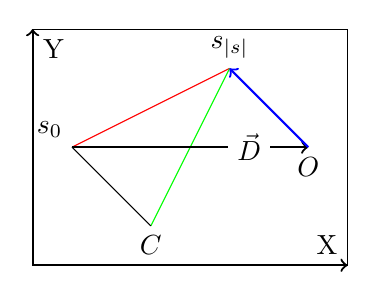
\begin{tikzpicture}
	\draw (-3.5,-1.5) rectangle (0.5,1.5);
	\draw[thick,->] (-3.5,-1.5) -- (0.5,-1.5) node[anchor=south east] {X};
	\draw[thick,->] (-3.5,-1.5) -- (-3.5,1.5) node[anchor=north west] {Y};

	\coordinate (A) at (-1,1);
	\coordinate (B) at (-3,0);
	\coordinate (C) at (-2,-1);
	\coordinate (O) at (0,0);

	\draw [red] (B) node[black, above left]{$s_0$} -- (A) node[black, above]{$s_{|s|}$};
	\draw [green] (A) -- (C)  node[black, below]{$C$};
	\draw (C) -- (B);
	\draw [thick, ->] (-3,0) -- (0,0) node [near end,fill=white]{$\vec{D}$} node [below] {$O$};
	\draw [thick, blue, ->] (O) -- (A);
	\end{tikzpicture}
	\caption{Szenario für das Vorgehen des GJK-Algorithmus und Veranschaulichung für ein ungenügendes Abbruchkriterium aus der Quelle \cite{gjk-casey}, dass den Algorithmus nicht am nächsten Merkmal zum Ursprung stoppt. Startpunkt $s_0$, maximaler Punkt in $\vec{D}$ ist $s_{|s|}$, stopp nach Quelle \cite{gjk-casey} mit (rot) $s_{new} = \{s_o, s_{|s|}\}$, da (blauer) Vektor $\vec{s_{|s|}}\circ\vec{D} < 0$. Tatsächliches nächstes Simplex zu $O$ ist aber (grün) $\overline{s_{|s|}C}$.}
	\label{fig:why_criteria}
\end{figure}

\begin{figure}
	\centering
	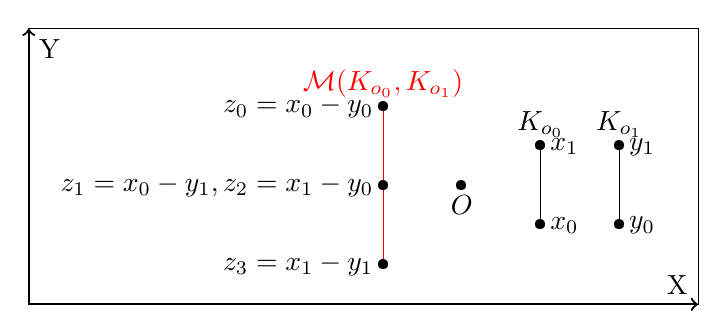
\begin{tikzpicture}



\draw (-5.5,-1.5) rectangle (3,2);
\draw[thick,->] (-5.5,-1.5) -- (3,-1.5) node[anchor=south east] {X};
\draw[thick,->] (-5.5,-1.5) -- (-5.5,2) node[anchor=north west] {Y};

\coordinate (VOaa) at (1,-0.5);
\coordinate (VOab) at (1,0.5);
\coordinate (VOba) at (2,-0.5);
\coordinate (VObb) at (2,0.5);

\coordinate (O) at (0,0);

\coordinate (A) at (-1,0);
\coordinate (B) at (-1,1);
\coordinate (C) at (-1,-1);

\draw [below](O) node[black]{$O$};
\draw (VOaa) -- (VOab);
\draw (VOba) -- (VObb);
\draw [red] (A) -- (B) -- (C);

\node at (O) {\textbullet};
\node at (A) {\textbullet};
\node at (B) {\textbullet};
\node at (C) {\textbullet};
\node at (VOaa) {\textbullet};
\node at (VOab) {\textbullet};
\node at (VOba) {\textbullet};
\node at (VObb) {\textbullet};

\node at (VOab)[above] {$K_{o_0}$};
\node at (VObb)[above] {$K_{o_1}$};

\node at (VOaa) [right]{$x_0$};
\node at (VOab) [right]{$x_1$};
\node at (VOba) [right]{$y_0$};
\node at (VObb) [right]{$y_1$};

\node at (B) [above, red]{$\mathcal{M}(K_{o_0}, K_{o_1})$};


\node at (B) [left]{$z_0=x_0-y_0$};
\node at (A) [left]{$z_1=x_0-y_1, z_2=x_1-y_0$};
\node at (C) [left]{$z_3=x_1-y_1$};

\end{tikzpicture}
	\caption{Minkowski-Differenz (rot) $\mathcal{M}(K_{o_0}, K_{o_1})$ mit markierten Punkten $\mathcal{M}(V_{o_0}, V_{o_1})$ mit mehreren nächsten Simplices $\{ \{z_1\},\{z_2\},\{z_0, z_3\},\{z_0,z_1\},\{z_1,z_2\}, ...\}$ zum Ursprung, sogar inklusive zweier deckungsgleicher punktförmiger Simplices mit kleinster Dimensionalität 0.}
	\label{fig:parfeat}
\end{figure}

\begin{enumerate}
\item In Schritt \ref{gjkstep3} wird eine Distanzverbesserung durch den neuen Punkt $s_{|s|}$ erwartet. Dadurch kann die Menge der nach ihrer Distanz zum Ursprung zu überprüfenden Simplices $s_{\alpha}$ eingeschränkt werden. Es werden nur Simplices überprüft, welche den neuen Punkt beinhalten. Die bereits durch $s$ bekannten Simplices sind vom Algorithmus zu einem vorigen Schritt bereits zu ihrer Distanz überprüft worden. Eine Wiederholung dieser Berechnung in diesem Durchgang wäre redundanter Aufwand. \cite{gjk-casey}
$$ s_{\alpha} = \mathcal{P}(s \cup \{s_{|s|}\}) \setminus \mathcal{P}(s)$$

\item Schritt \ref{gjkstep3} kann durch die Suche nach der relativen Position des Ursprungs zum bekannten Simplex durch sukzessive geometrische Raumaufteilung realisiert werden \cite{gjk-casey}. Alle Punkte des Raums können mathematisch einem nächsten Simplex zugewiesen werden. Die Zugehörigkeit zu einem Raumteil kann durch Skalarprodukte und Kreuzprodukte ermittelt werden. (Beispiele in Quelle \cite{gjk-casey})

\item Für die Berechnung von Minkowski-Punkten $\mathcal{M}(V_{o_0}, V_{o_1})$ wird ein Generator-Muster verwendet, welches zum Minkowski-Punkt Indices der verwendeten Eckpunkte der Ursprungsmodelle $V_{o_0}$ und $V_{o_1}$ mitführt. Damit können durch den Erhalt des nächsten Simpex $s$ die an der Kollision beteiligten Merkmale/Simplices der Eingabeobjekte rückwirkend ermittelt werden.

\item Die Quelle \cite{gjk-casey} zeigt ein mögliches verfrühtes Abbruchkriterium des Algorithmus zwischen Schritten \ref{gjkstep2} und \ref{gjkstep3}. Dadurch kann verfrüht die Exklusion des Ursprungs festgestellt werden.
$$\vec{s_{|s|}} \circ \vec{D} < 0 \Rightarrow O \notin \mathcal{M}(K_{o_0, t}, K_{o_1, t})$$
Daraus kann hinsichtlich der Distanz $>0$ zwischen Minkowski-Differenz und Ursprung keine genauere Aussage gemacht werden.
Die Grafik \ref{fig:why_criteria} zeigt dafür ein widersprüchliches Beispiel.
Unter Umständen ist es die undokumentierte Intention der Quelle \cite{gjk-casey} nur eine Implementierung zu liefern, die keine minimale Distanz oder nächste Simplices ermittelt, sondern nur ob ein Schnitt existiert, oder nicht. Die Ausschreibungen der Quelle als Implementierung des GJK-Algorithmus ist daher irreführend.

\item Das Abbruchkriterium des Algorithmus verlangt die Berechnung und den Vergleich aller Distanzen neuer Simplices $s_{\alpha}$. Es wurde, ganz im Sinne der Quelle \cite{gjk-casey}, ohne Erfolg versucht ein Abbruchkriterium zu finden, bei der diese Distanzberechnung nicht stattfindet und welches dieses ersetzen kann.
\begin{enumerate}
	\item Ist der neue gefundene Punkt $s_{|s|}$ bereits in $s$ bekannt, kann keine Distanzverbesserung mehr erzielt werden, da keine neuen, dem Algorithmus unbekannten Simplices nun bekannt werden.
	 $$s_{|s|} \in s \Rightarrow distance(K_{o_0}, K_{o_1}) = distance(s, O) = d_{min}\text{(\textbf{RETURN})}$$ 
	\item Durch den neuen Punkt $s_{|s|}$ gezogene Kantenvektoren zu bereits bekannten Simplexpunkten $\vec{s_{|s|}v}, v\in s$ sollen eine klare Erweiterung in Suchrichtung $\vec{D}$ darstellen, was durch das Skalarprodukt ermittelbar ist $\vec{D} \circ \vec{s_{|s|}v} < 0$.
\end{enumerate}

Bei Versuchen mit diesen Abbruchkriterien konvergierte der Algorithmus regelmäßig nicht. Es wurden falsche Annahmen getroffen:
\begin{enumerate}
\item Das nächste Simplex zum Ursprung ist eindeutig.\\
Die Minkowski-Summe produziert keine Hüllenobjekte, nur konvexe Vertex-Meshes. Es können daraus mehrere nächste Simplices zum Ursprung generiert werden, wie die Abbildung \ref{fig:parfeat} zeigt. Das Problem kann dann auftreten, wenn Merkmale der Objekte z.B.~komplanar sind.
\item Verwendete Funktionen sind ausreichend genau.\\
Theoretisch sollten komplanare Merkmale dieselbe neue Suchrichtung $\vec{D}$ in Schritt 8.~erzeugen. Der neue Punkt $s_{|s|}$ ist dabei dann eindeutig (maximales Skalarprodukt im Konvexen). Das scheint durch Berechnungsungenauigkeiten, insbesondere im Kreuzprodukt, nicht der Fall zu sein. 
\end{enumerate}

Die Uneindeutigkeit der nächsten Simplices und Berechnungsungenauigkeiten führten im Algorithmus zu wiederholt denselben Belegungen von $s$ und somit zu Endlosschleifen.\\
Nur Abbruchkriterium (a) arbeitet nicht mit dem Kreuzprodukt, führte in allen Tests immer erfolgreich zur Konvergenz und wird daher letztendlich verwendet.
Die selbst ermittelten Abbruchkriterien eignen sich also nur als unzuverlässige frühe Abbruchkriterien, die das bekannte Abbruchkriterium durch die minimale Distanz nicht vollständig ersetzen könne. Ob die Vorschaltung dieser Verfahren einen Vorteil bietet müsste eine praktische Messung (Benchmark) zeigen, dessen Aufwand für den Rahmen dieses Projekts jedoch als zu aufwändig eingeschätzt wird.
\end{enumerate}

\subsubsection{Umsetzung eines Intrusionsalgorithmus mit GJK}
GJK löst das Schnittproblem zu einem bestimmten Zeitpunkt, bzw. Simulationsstatus der Objekte. Über die Suche der ersten Nullstelle des GJK als Distanzfunktion während eines Ticks kann die Zeit einer Erstkollision bestimmt werden, um zusätzlich das Intrusionsproblem zu lösen.
Ein Nullstellen-/Wurzelsuchverfahren hat zudem den Vorteil, dass es unabhängig von der Bewegungsart der Objekte ist. Animation, Rotation oder beliebige Transformation ist prinzipiell denkbar, solange die Bewegung durch die Distanz abstrahiert werden kann und die Distanzfunktion stetig ist.\\
Es sind prinzipiell viele Wurzelsuchverfahren bekannt. Viele werden jedoch durch den Umstand einer niemals negativen Distanz in $\mathbb{R}^+_0$ verkompliziert.\\
Die zusätzliche Berechnung negativer Distanz, also eine Penetrationstiefe, wurde an dieser Stelle nicht weiter untersucht.\\
Vor allem bei rotierenden Objekten werden Hürden ersichtlich:
Bei Rotierenden Objekten nimmt die Distanzfunktion die Form einer Schwingung an, wodurch das Nyquist-Shannon-Abtasttheorem \cite{nyquist} gilt. Es gilt also auch bei diesem Verfahren eine Einschränkung der Rotationsgeschwindigkeit oder Verlust der Zuverlässigkeit des Verfahrens selbst. Es bestätigt sich hier wieder die bereits in Abschnitt~\ref{sec:linear_int} gemachte Einschätzung von Rotation als limitierenden Faktor. Anders als dort kann bei diesem Verfahren jedoch durch die nun bekannte Abstraktion über die Distanz besser auf die Limitation eingegangen werden.\\
Es wurde ein triviales Wurzelsuchverfahren implementiert, welches zunächst mit einer einstellbaren Abtastrate $r_{sample}$  pro Ticks nach einer Distanz $= 0$ sucht. Das erste zeitliche Auftreten eines solchen Ereignisses wird dann weiter zur binären Suche des durch Samples eingegrenzten Zeitabschnitts verwendet, um den bei der Intrusion geforderten Zeitpunkt mit einer bestimmten Genauigkeit $\epsilon_t$ festzustellen.\\
Wir erfahren ebenfalls Begrenzungen durch die Genauigkeit von Floating-Point-Datentypen, die aus der verwendeten Kollisionsauflösung ersichtlich werden. Nach der Nullstellensuche wird das Objekt auf den letzten ermittelbaren Zustand vor der Kollision gesetzt, und Bewegungen absolut eliminiert. Zu erwarten wären Kollisionspaare mit infinitesimal kleinem Abstand zueinander, nachdem eine Kollision geschehen ist.\\
Tatsächlich variieren Abstände nach der Kollision jedoch erheblich im Bereich von kleiner 10\% der Objektgröße, besonders bei Objekten mit ursprünglich hoher Geschwindigkeit und Drehgeschwindigkeit. Die Variation kann auf das kleinste Zeitintervall in der Nullstellensuche zurückgeführt werden, welches bei hohen Geschwindigkeiten offenbar nicht klein genug ist, um einen Zustand der kollidierenden Objekte mit annähernd infinitesimal kleinen Abstand zu ermitteln.\\

\subsubsection{Komplexität}
Die Komplexität des Verfahrens hängt von der Komplexität der Teilalgorithmen ab:
\begin{enumerate}
\item die Anzahl der konvexen Partitionen der Objekte $\mathcal{O}(|P_{o_0}|\cdot |P_{o_1}|)$
\item der Komplexität des Wurzelsuchverfahrens:\\
 Für das in diesem Projekt verwendete Verfahren ist dies $$\mathcal{O}(r_{sample} + \log_{2}(\frac{(t_1 - t_0)}{r_{sample}\epsilon_t} ))$$
\item der Komplexität von GJK:\\
Ein Durchlauf der in Schritt \ref{gjkloop} angelegten Schleife bringt die Komplexität der Zwischenschritte mit sich. Die nicht-trivial Konstanten sind:
\begin{enumerate}
\item Schritt \ref{gjkstep2} $\mathcal{O}(|\mathcal{M}(V_{o_0}, V_{o_1})|) = \mathcal{O}(|V_{o_0}|\cdot |V_{o_1}|)$.
\item Schritt \ref{gjkstep3} $\mathcal{O}(\mathcal{P}(s)) = \mathcal{O}(2^{|s|})$, aber $|s| \leq 4 \Rightarrow \mathcal{O}(2^4) = \mathcal{O}(16)$.
\end{enumerate}
Die Komplexität innerhalb der Schleife hängt also hauptsächlich von der Beschaffenheit der Objekte, bzw.~ihrer Minkowski-Differenz ab.\\
Wie viele Schleifendurchläufe benötigt werden kann theoretisch nur durch $|\mathcal{M}| = |V_{o_0}|\cdot |V_{o_1}|$ eingegrenzt werden.
\end{enumerate}
Insgesamt entsteht in diesem Projekt die Komplexität 
$$\mathcal{O}(|P_{o_0}|\cdot |P_{o_1}| \cdot  \left( r_{sample} + \log_{2}\left(\frac{t_1 - t_0}{r_{sample}\epsilon_t}\right)\right) \cdot  |V_{o_0}|\cdot |V_{o_1}| )$$


\subsection{Vergleiche, Fazit \& Ausblick}
\label{sec:ausblick}
Die hier vorgestellten Verfahren der linearen Interpolation und GJK erreichen sehr Unterschiedliche Ziele mit unterschiedlichen Voraussetzungen und lassen sich daher nur schlecht vergleichen.\\
Das vermehrte Potential zur Optimierung wird in GJK gesehen.
Beispiele/Experimente für Optimierungen des GJK im Ausblick:
\begin{enumerate}
\item konvexe Partitionen könnten vorgefiltert werden, wie z.B. durch Behandlung als quasi eigene Entität in Abschnitt~\ref{sec:l1}. Die dort beschriebenen Möglichkeiten geben dabei Aufschluss über die hier verwendbaren Optionen.
\item Die Urquelle \cite[p.196, math. Indices (16), (17), (21)]{gjk} beschreibt die Möglichkeit der Optimierung der Suche eines neuen maximalen Punktes der Minkowski-Differenz in einer Richtung (Algorithmus Schritt \ref{gjkstep2}) von $\mathcal{O}(|V_{o_0}|\cdot |V_{o_1}|)$ auf $\mathcal{O}(|V_{o_0}|+|V_{o_1}|)$. Die Optimierung würde die direkte Eingabe von Ursprungsobjekten (Partitionen) $o_0, o_1$ in den Algorithmus erfordern. Das Design wurde jedoch zu einem frühen Zeitpunkt bereits auf die Eingabe der Minkowski-Differenz festgelegt. Die Entscheidung, einen Generator für Minkowski-Punkte als Eingabe für den GJK-Algorithmus zu verwenden, erweist sich hier als unvorteilhaft, da die involvierten Prozesse nun strukturelle Hindernisse zur einfachen Umsetzung dieser Optimierung erzeugen.
\item Einführung partieller Ordnungen zwischen Eckpunkten an einem Körper, um die Suche in Schritt \ref{gjkstep2} noch weiter auf $\mathcal{O}(\log(|V_{o_0}|)+log(|V_{o_1}|)$ zu optimieren.
\item dynamische Auswahl besserer Wurzelsuchverfahren (vgl.~\cite{gdc-physics}), auch anhand von Details zu Objekten (Rotationsgeschwindigkeit, Varianz von Vektorlängen zu Eckpunkten, etc.)
\end{enumerate}
Unter diesen Umständen sollte GJK den in Abschnitt \ref{sec:linear_int} gezeigten Algorithmus auch in dessen eingeschränkten Anwendungsbereich in Punkten Komplexität gleichziehen oder gar untertreffen:
\begin{itemize}
\item Statisches konvexes Objekt $o_0$ wird von Projektil/Punktförmigen Objekt $o_1$ getroffen, d.h. es liegt nur minimale konvexe Partitionierung vor: $|P_{o_o}| = |P_{o_1}| = 1$
\item Eingrenzung der Wurzelsuche durch Differenzierbarkeit der linearen Projektilbewegung durch Annäherung des Suchraums auf $t_{\alpha}, t_{\omega}$ in $\mathcal{O}(4)$ mit 4 Samples von $t_0, t_0+\epsilon_{t}, t_1, t_1 - \epsilon_{t}$ in schnellerer Zeit  möglich.
\end{itemize}
\begin{gather*}
\mathcal{O}(~1\cdot 1\cdot 4\cdot \left(r_{sample} + \log_{2}\left(\frac{(t_{\omega} - t_\alpha)}{r_{sample}\epsilon_t}\right)\right)\cdot (\log(|V_{o_0}|)+log(|V_{o_1}|))~) \\
\stackrel{?}{<}\\
 \mathcal{O}(|V_{o0}|\cdot  |A_{o1}| + |V_{o1}|\cdot |A_{o0}| + |E_{o0}| \cdot  |E_{o1}|)
\end{gather*}

Der GJK ist theoretisch für $m\in\mathbb{N}$ Dimensionen definiert \cite{gjk}. Durch die Behandlung von Objekten während eines Ticks als 4-dimensionale kompakte Menge $\bigcup_{t \in \Upsilon_{\delta_i}} K_{o,t}$ könnte der zeitunabhängige Schnitt ermittelt werden um entsprechend vorzufiltern. Besonders im Kontext linearer Bewegungen als Vorfilterung im Kontext zu Abschnitt \ref{sec:linear_int} wäre die Ermittlung der Eckpunkte des durchlaufenen Volumens für einen vorgeschalteten GJK einfach $V_{o, t_0} \cup V_{o, t_1}$, also der Aufwand einer einzigen Transformation pro Objekt.\\

Hinsichtlich der Optimierungsmöglichkeiten mag sich weiterer Zeitaufwand daher durchaus lohnen.\\

Ohne die Bemühungen zu Vorfilterung in Abschnitt \ref{sec:l1}, so zeigen Tests, wäre die GJK-Routine alleine für Echtzeitfähigkeit nicht ausreichend. Wir messen 650ms gesamte Rechenzeit für ca.~100 Objekte ohne AABB Vorfilterung während beliebige Vorfilterungsmethoden diese Zeit bereits auf ca.~6ms reduziert. Die Einschätzung zur Echtzeitfähigkeit gilt zum derzeitigen Stand und schätzungsweise auch für die zu erwartende Optimierungsfähigkeit modellgenauer Kollisionsverfahren für die Zukunft des Projektes.